\section {Cronograma de actividades}
Durante el primer semestre se recolectará información de forma aislada así como integrada con aplicaciones afines al proyecto, en el segundo se construirán los modelos para la obtención de la base de datos. En la segunda mitad se llevarán a cabo actividades de desarrollo, en tercer semestre se obtendrá el conjunto de palabras para extender la búsqueda y estimar modelos de regresión, y se realizará una búsqueda correlacionada complementaria. En cuarto semestre se obtendrán nuevos modelos de regresión lineal utilizando los datos obtenidos en la búsqueda previa y se realizarán pruebas de hipótesis del modelo anterior para obtener mejores estimadores, se construirán elementos gráficos 
\begin{figure}[H]\centering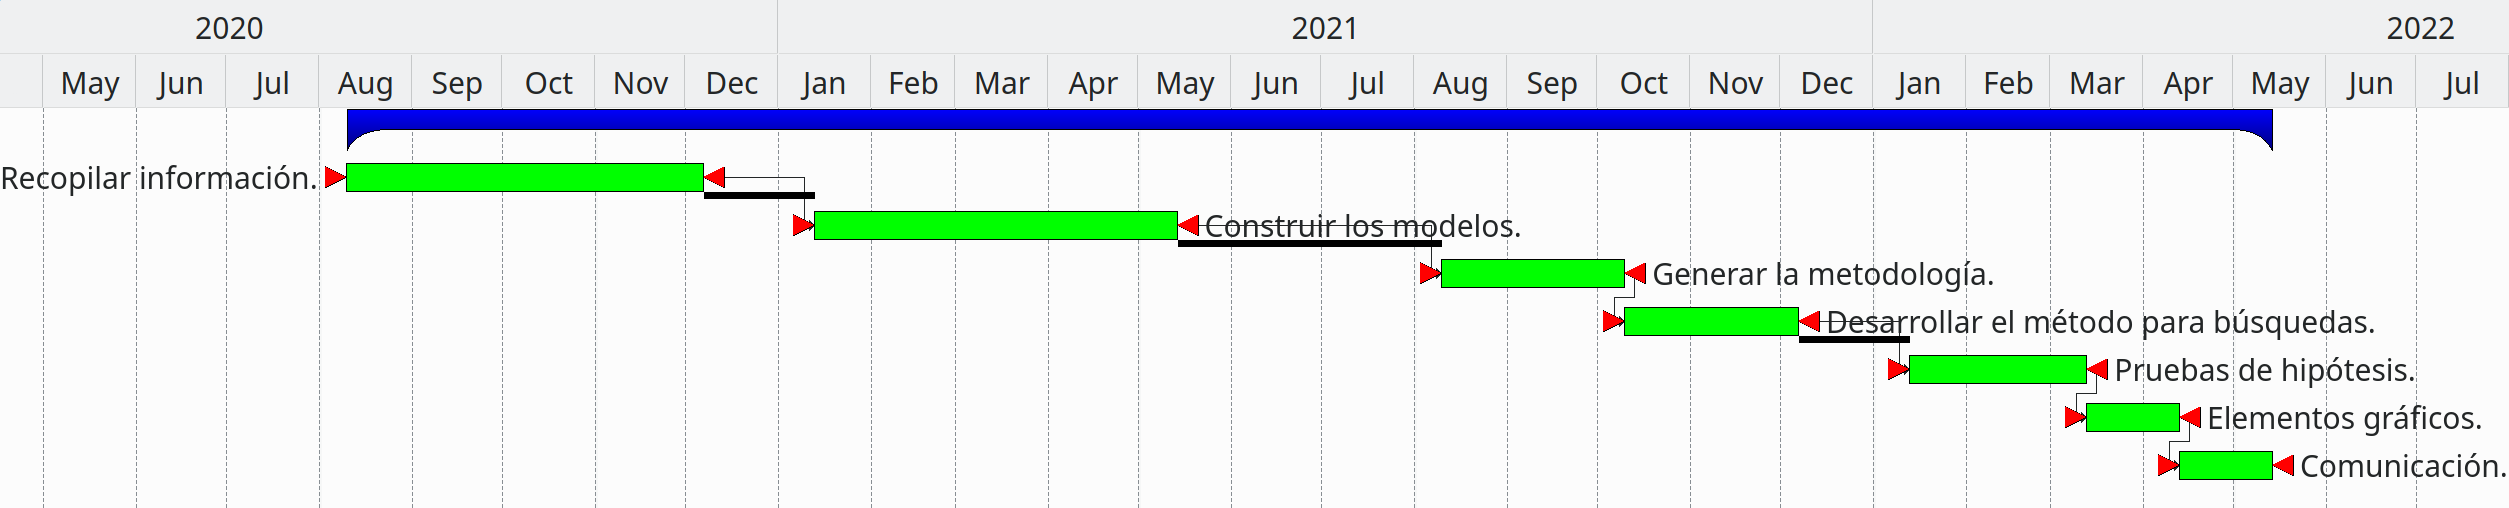
\includegraphics[width=1\linewidth]{gantt.png}\end{figure}